\documentclass[10pt,a4paper]{article}

\usepackage[utf8]{inputenc}		% Configuro la codificación
\input{.command.tex}
% En el siguiente archivo se configuran las variables del trabajo práctico
%% \providecommand es similar a \newcommnad, salvo que el primero ante un 
%% conflicto en la compilación, es ignorado.

% Al comienzo de un TP se debe modificar los argumentos de los comandos

\providecommand{\myTitle}{PROYECTO FINAL}
\providecommand{\mySubtitle}{Amplificador de audio de potencia Clase G alternativa}

\providecommand{\mySubject}{Diseño de Circuitos Electrónicos (86.10)}
\providecommand{\myKeywords}{UBA, Ingeniería, C2}

\providecommand{\myTutor}{-}
\providecommand{\myAuthorSurname}{Alonso, Manso, Russo, Zuccolo}
\providecommand{\myTimePeriod}{Año 2018 - 2\textsuperscript{do} Cuatrimestre}

% No es necesario modificar este %%%%%%%%%%%%%%
\providecommand{\myHeaderLogo}{header_fiuba}
%%%%%%%%%%%%%%%%%%%%%%%%%%%%%%%%%%%%%%%%%%%%%%%%

% Si se utilizan listings, definir el lenguaje aquí
\providecommand{\myLanguage}{matlab}

% Crear los integrantes del TP con el comando \PutMember donde
%%		1) Apellido, Nombre
%%		2) Número de Padrón
%%		3) E-Mail
\providecommand{\MembersOnCover}[0]
{		
		\PutMember{Alonso, Gustavo Gabriel} {96119} {gustavoalon19@gmail.com}
		\PutMember{Manso, Juan} {96133} {juanmanso@gmail.com}
		\PutMember{Russo, Nicolas Emanuel} {93211} {nicolasrusso291@gmail.com}
		\PutMember{Zuccolo, Florencia} {96628} {florenciaz618@gmail.com}
}

\providecommand{\myGroupNumber}{10}

\Pagebreaktrue		% Setea si hay un salto de página en la carátula
\Indextrue
\Siunitxtrue			% Si quiero utilizar el paquete, \siunixtrue. Si no \siunixfalse
\Todonotestrue		% Habilita/Deshabilita las To-Do Notes y las funciones \unsure, \change, \info, \improvement y \thiswillnotshow.
\Listingsfalse
\Keywordsfalse
\Putgrouptrue		% Habilita/Deshabilita el \myGroup en los headers
\Videofalse
\Tutorfalse
				% Archivo con los comandos globales como Título y autores
%Preambulo para articulo científico de LaTeX

\usepackage[a4paper,left=3cm,right=3cm,bottom=3.5cm,top=3.5cm]{geometry} 	% Configuro la geometría del papel
%\usepackage{microtype}								% Mejora el "spacing" de las palabras
\usepackage[spanish]{babel} 							% Compatibilizo los signos del español
	\addto\captionsspanish{\renewcommand{\tablename}{Tabla}}		%% Redefino nombres preestablecidos por Babel
	\addto\captionsspanish{\renewcommand{\listtablename}{Índice de tablas}}	%% y así en vez de Cuadro dirá Tabla.
\usepackage{amsmath, amsfonts, amssymb}						% Entornos matemáticos, fuentes y símbolos
\usepackage{graphicx}								% Necesario para insertar figuras
\usepackage{fancyhdr}								% Para manipular headers y footers
\usepackage[usenames,dvipsnames]{color}						% \color{color deseado} {lo que querés que tenga color}
\usepackage{subcaption}								% Permite captions del tipo 1a, 1b
\usepackage{multirow}								% Para tablas
\usepackage{multicol}
%\usepackage{slashbox}								% Cuadro divido en tablas
\usepackage{diagbox}
\usepackage{float}
\usepackage{booktabs}								% Permite hacer tablas sin separadores en el medio
\usepackage[table,xcdraw]{xcolor}						% Para colorear tablas

% Para video
\ifVideo
	\usepackage{media9}
	\addmediapath{./../reportes/}
\fi

%\usepackage{times}
%\usepackage{mathtools}
%\usepackage{upgreek} % letras griegas sin cursiva
%\usepackage{cancel}
\usepackage{rotating}
\usepackage{tikz}
\usepackage{pgfplots}
%	\pgfplotsset{compat=1.12}
	\usetikzlibrary{plotmarks}% matlab2tikz
\usepackage{grffile}% matlab2tikz 
	\usetikzlibrary{calc,patterns,decorations.pathmorphing,decorations.markings}

\ifListings
	\usepackage{listings}

	\providecommand{\lstinputpath}[1]{\lstset{inputpath=#1}}

%	\input{.lst_default.tex}
	\input{.lst_matlab.tex}
%	\input{.lst_c.tex}
%	\input{.lst_c++.tex}
	
% 	\input{.lst_pseudocode.tex}


\fi

\ifSiunitx
\usepackage{siunitx}											% Unidades: \SI {cantidad} {\unidad} (necesita texlive-science)
	\sisetup{load-configurations = abbreviations}							% Habilita poner \cm en vez de \centi\metre
	\sisetup{output-decimal-marker = {,}}									% Cambia los puntos decimales por comas
	\sisetup{per-mode = fraction}											% Pone las unidades como fracción
	\sisetup{quotient-mode = fraction}										
\fi


\ifTodonotes
\usepackage{xargs}
\usepackage[colorinlistoftodos,prependcaption,textsize=tiny]{todonotes}


	\newcommandx{\Juan}[2][1=]{\todo[linecolor=red,backgroundcolor=red!25,bordercolor=red,#1]{#2}}
	\newcommandx{\Flor}[2][1=]{\todo[linecolor=blue,backgroundcolor=blue!25,bordercolor=blue,#1]{#2}}
	\newcommandx{\Gus}[2][1=]{\todo[linecolor=green,backgroundcolor=green!25,bordercolor=green,#1]{#2}} % OliveGreen
	\newcommandx{\Nico}[2][1=]{\todo[linecolor=yellow,backgroundcolor=yellow!25,bordercolor=yellow,#1]{#2}}
	\newcommandx{\thiswillnotshow}[2][1=]{\todo[disable,#1]{#2}}
\fi


\usepackage{placeins}														
		\let\Oldsection\section												%% Permite que los flotantes (como figuras) no aparescan
	\renewcommand{\section}{\FloatBarrier\Oldsection}						%% antes o después de su sección correspondiente.
		\let\Oldsubsection\subsection
	\renewcommand{\subsection}{\FloatBarrier\Oldsubsection}		
		\let\Oldsubsubsection\subsubsection
	\renewcommand{\subsubsection}{\FloatBarrier\Oldsubsubsection}
\usepackage{hyperref}														% Debe ser agregado al final del preambulo

\hypersetup
{    bookmarks=true,         % show bookmarks bar?
     unicode=false,          % non-Latin characters in Acrobat’s bookmarks
     pdftoolbar=true,        % show Acrobat’s toolbar?
     pdfmenubar=true,        % show Acrobat’s menu?
     pdffitwindow=false,     % window fit to page when opened
     pdftitle={\myTitle},    		 % title
     pdfauthor={\myAuthorSurname},   % author
	 pdfcreator={\myAuthorSurname},	 % creator = author
     pdfsubject={\mySubject},		 % subject of the document
     pdfkeywords={\myKeywords},
     colorlinks=true,        % false: boxed links; true: colored links
     linkcolor=black,        % color of internal links (change box color with linkbordercolor)
     citecolor=black,        % color of links to bibliography
     filecolor=magenta,      % color of file links
     urlcolor=cyan           % color of external links
}

%Configuro la pagina con los encabezaos y pies de paginas
\pagestyle{fancy}										% Para agregar encabezados y pie de paginas	
%\lhead{\mySubject}										% Encabezado izquierdo
\lhead{DCE (86.10)}
\rhead{\includegraphics[scale=0.15]{\myHeaderLogo}} 	% Encabezado derecho (logo de la FIUBA)	
\ifPutgroup
\chead{\texttt{Grupo Nº\myGroupNumber} \\ \textit{\footnotesize{\myTimePeriod}}}
\fi				

%% Este archivo contiene las funciones auxiliares para escribir en LaTeX
%% Dichas funciones resuelven la sintaxis de generar figuras, por ejemplo,
%% dejando el código más compacto y facilitando la corrección del mismo.



% Comando para graficar eps. 1er arg, escala. 2do, ruta. 3ro, caption. 4to, label.
\providecommand{\HgraficarEPS}[4]{
			\begin{figure}[h!]
				\centering
					\scalebox{#1}{\input{#2}}
					\caption{#3}
					\label{#4}
			\end{figure}

}

\providecommand{\HgraficarPNG}[4]{
			\begin{figure}[h!]
				\centering
					\includegraphics[scale=#1]{#2}
					\caption{#3}
					\label{#4}
			\end{figure}

}


% Comando para graficar eps en el lugar previsto.
\providecommand{\graficarEPS}[4]{
			\begin{figure}[h]
				\centering
					\scalebox{#1}{\input{#2}}
					\caption{#3}
					\label{#4}
			\end{figure}

}

\providecommand{\graficarPNG}[4]{
			\begin{figure}[h]
				\centering
					\includegraphics[scale=#1]{#2}
					\caption{#3}
					\label{#4}
			\end{figure}

}

\providecommand{\underuparrow}[2]{\underset{\underset{#2} \uparrow} #1 }

\providecommand{\cltext}[2]{\color{#1}{\huge{#2}}}
\providecommand{\cstext}[2]{\color{#1}{\large{#2}}}

\providecommand{\lsi}[1]{\large\si{#1}}
\providecommand{\lsio}[0]{\large\si{\ohm}}
\providecommand{\lsiv}[0]{\large\si{\volt}}
\providecommand{\lsia}[0]{\large\si{\ampere}}
\providecommand{\lSI}[2]{\large\SI{#1}{#2}}


		% Se proveen un conjunto de funciones extras

% Defino el path de los includegraphics
\graphicspath{{./Figuras/}}		% Directorio que contiene los graficos

% Defino el path para los input de .tex y de .eps
\makeatletter
\def\input@path{{./Figuras/}{./Secciones/}{./Cover_page/}{../Octave/graficos/}}
\makeatother

% Defino el path del listings
\ifListings
%% Cambiar el nombre de la carpeta si se utilizan Listings
	\lstinputpath{{../Octave/}}
\fi

\definecolor{myred}{rgb}{0.5,0,0}
\definecolor{mygreen}{rgb}{0,0.5,0}



\begin{document}
		% Carátula (formal o simple,_formal o _simple respectivamente) con Resumen
		% incluido e Índice (si es necesario configurar en config.tex) del informe
		\begin{titlepage}
	
		\thispagestyle{empty}

		\begin{center}
			
\includegraphics[scale=0.3]{fiuba}\\
			\large{\textsc{Universidad de Buenos Aires}}\\
			\large{\textsc{Facultad De Ingeniería}}\\
			\small{\myTimePeriod}
		\end{center}

		\vfill

		\begin{center}
			\Large{\underline{\textsc{\mySubject}}}
		\end{center}

		\vfill

		\begin{tabbing}
			\hspace{2cm}\=\+\myTitle\\
				TEMA: \mySubtitle\\
				TUTOR: \myTutor\\
				FECHA: \today\\
				\ifPutgroup
				GRUPO: \texttt{\myGroupNumber}\\
				\fi

			\\
				\MembersHeader
				\MembersOnCover	
		\end{tabbing}

		\begin{abstract}
			% Ejemplo de Resumen
%% MANTENER EL NOMBRE %%
El presente informe expone el proceso de diseño y construcción de un equipo electrónico partiendo de ciertas especificaciones.

		\end{abstract}

	\ifKeywords
		\begin{center}
			\emph{Palabras Clave: \myKeywords}
		\end{center}
	\fi	

		\vfill
	
\end{titlepage}

\ifPagebreak
	\thispagestyle{empty}
	\ifIndex
		\tableofcontents
%		\listoffigures
%		\listoftables
	\fi

	\pagebreak
\fi


	\setcounter{page}{1}

	\part{Introducción}\label{part:intro}

		\section{Objetivos}\label{sec:obj}
			
%	Las señales de audio tienen una relación de pico/valor medio elevado, estando la mayor parte del tiempo en valores bajos.

	El trabajo consiste en la confección de un amplificador de audio tanto en su forma teórica como práctica; una vez determinados los valores de los componentes a partir de un análisis teórico y posterior simulación, se procede a armar el mismo de forma discreta y realizar distintas mediciones para compararlas con los datos previamente obtenidos. \\ 

	A continuación se analiza su comportamiento y se detalla cada parte del circuito, explicando el propósito de cada componente y el valor elegido para su óptimo funcionamiento.


		\section{Requerimientos}\label{sec:req}
			El amplificador de audio a diseñar debe cumplir las siguientes especificaciones:

\begin{itemize}
	\item Topología de la etapa de salida Clase G alternativa.
	\item Tensión de alimentación $\pm \SI{30}{\volt}$ con una variación de \SI{5}{\volt}.
%	\item Potencia de salida nominal de \SI{39}{\watt} sobre \SI{8}{\ohm} a \SI{1}{\kilo\hertz} con $THD<0,02\%$.
	\item Potencia de salida nominal de \SI{40}{\watt} sobre \SI{8}{\ohm} a \SI{1}{\kilo\hertz} con $THD<0,02\%$.
	\item Potencia de salida a \SI{1}{\watt} sobre \SI{8}{\ohm} con $THD<0,01\%$. 
	\item Respuesta en frecuencia \SI{20}{\hertz} a \SI{20}{\kilo\hertz}.
	\item Tensión de \textit{offset} en la salida en continua \SI{5}{\milli\volt}.
	\item \textit{Slew Rate} $\approx$ \SI{10}{\volt\per\micro\second}.
	\item Distorsión IMD cercana al 1\%.
	\item Impedancia de entrada del orden de \SI{100}{\kilo\ohm}.
	\item Impedancia de salida del orden de los \SI{}{\milli\ohm}.
	\item Factor de amortiguamiento del orden de 500.
	\item Margen de fase mayor que \SI{45}{\degree}.
\end{itemize}


%
%	\begin{table}[h!]
%		\centering
%		\begin{tabular}{*{2}{c}}
%			\toprule
%			Tipo de especificación & Valor\\
%			\midrule
%			$\pm V_{CC}$			& $\pm$\SI{30}{\V} con tolerancia de $\pm$\SI{1}{\V}\\
%			Respuesta en frecuencia		& \SI{20}{\Hz} a \SI{20}{\kHz}\\
%			Ancho de banda de potencia	& \SI{20}{\Hz} a \SI{20}{\kHz}\\
%			Rango dinámico			& Mínimo = \SI{40}{\dB} para reproducir vinilos\\
%			Distorsión armónica total (\emph{THD})& Mínimo = 1\%\\
%			Relación señal a ruido (\emph{SNR})& \SI{60}{\dB}\\
%			Sensibilidad			& 1 Vrms\\
%			\emph{Slew Rate}		& \SI{15}{\micro\V\per\second}\\
%			\emph{DC Offset}		& Máximo = \SI{1}{\mV}\\
%			Impedancia de entrada		& $R_{in} \approx \SI{10}{\kilo\ohm}$\\
%			Impedancia de salida		& $R_{out} \approx \SI{10}{\milli\ohm}$\\
%			Factor de amortiguamiento	& $FA \approx 500$\\
%			Margen de fase			& $\varphi_m= \SI{60}{\degree}$\\
%			Margen de ganancia		& Sólo que sea positivo para que sea estable\\
%			Potencia nominal (sin exigir mucho) & Suponiendo que no le dan con todo, todo el tiempo\\
%			Potencia máxima			& Para 25V\\
%			\bottomrule
%		\end{tabular}
%	\end{table}
%
%
%	Poner las bases de los comporadares en Vout en vez de la salida de la 2nda.
%	Bajar el Vth
%	Ver qué queda en la corriente de salida a partir de la distorsión
%	Bajar la resistencia de emisor del comparador para tener menos corriente.
%	Ver las corrientes que necesitan los tr de salida.
%	
%


	\part{Diseño conceptual}\label{part:concept}

		\section{Alternativas de diseño}\label{sec:alt}
			
	A partir del análisis realizado sobre el amplificador \emph{Turner 730} se ve que una implementación posible de la etapa de entrada es un emisor común. Se considera la alternativa de utilizar un par diferencial. A pesar de la dificultad propia del balanceo del par diferencial (selección de componentes similares, cargas, fuentes de corriente, etc.), las ventajas del mismo son mucho mayores al emisor común que se utilizaba en los \emph{70} dada la escasez de transistores. Entre las ventajas se destaca la baja tensión de corrimiento $V_{off}$; las corrientes no fluyen por el lazo de realimentación; linealidad superior a la entrada con 1 solo transistor; buen acoplamiento térmico.\\

	Por otro lado, para la implementación de los comparadores encargados de la conmutación de las fuentes externas de la etapa de salida clase G alternativa se consideraron amplificadores operaciones y un par diferencial discreto. Los amplificadores operacionales facilitan la implementación del circuito, pero dificulta la producción dada la escasez o falta de provisión de los mismos. La solución es realizar un diseño sencillo con transistores discretos de un par diferencial que a su vez es más ajustable dado que el diseño es propio y se puede personalizar el comparador a la medida de las necesidades del dispositivo.\\

	\Juan{Qué alternativa sería 'Separación de VAS con corriente de polarización de etapa de salida (separada por un capacitor)'?}


%	- Comparadores: utilización de operacionales en vez del par diferencial discreto. Componentes difíciles de conseguir
%	
%	- Separación de VAS con corriente de polarizacion de etapa de salida (separada por un capacitor)
%	
%	- Multiplicador de VBE doble.
%	
%	\Juan{Hacer la tabla en internet}
%	\begin{table}[h!]
%		\centering
%		\begin{tabular}{*{4}{c}}
%			\toprule
%			Etapa                                  & Alternativa & Ventajas & Desventajas \\ 
%			\midrule
%			\multirow{2}{*}{Comparador de entrada} &             &          &             \\ %\cmidrule(l){2-4} 
%	&\colortab Par diferencial             &          &             \\
%			\midrule
%			\multirow{2}{*}{VAS} &             &          &             \\ %\cmidrule(l){2-4} 
%			                                       &             &          &             \\
%			\midrule
%			\multirow{2}{*}{Etapa de salida} & Clase G            &          &             \\ %\cmidrule(l){2-4} 
%							 &  \colortab Clase G alternativa           & \colortab Menor distorsión	& \colortab Diseño más complejo\\
%			\midrule
%			\multirow{2}{*}{Fuente de corriente} & FES	& Simple	& Error apreciable, malo bajo ripple             \\ %\cmidrule(l){2-4} 
%							&\colortab FES corregida	& \colortab Más estable vs ripple	& \colortab Más componentes \\
%			\bottomrule
%		\end{tabular}
%	\end{table}
%	
%	Carga FES versus bootstrap en el VAS. El bootstrap es dependiente de la ganancia de la etapa de salida y esta puede variar por la carga utilizada. Otra contra es la corriente de polarizacion varia segun varie la fuente 
%	Cascode versus colector común pre emisor común. Cascode permite VAS con alto beta y buena respuesta en frecuencia. Colector común es más simple y facil de diseñar.


		\section{Diagrama en bloques}\label{sec:bloques}
			\HgraficarEPS{0.5}{bloques}{Diagrama en bloques}{fig.bloques}

	\Juan{Tal vez hacer los bloques que marcamos después más adelante.. ¿?}
	En la Figura \ref{fig.bloques} se muestran los bloques principales de un amplificador de audio, que consiste en tres etapas, cada una de ellas con cierta funcionalidad.

\begin{itemize}
	\item \textbf{Comparador:} es un amplificador de transconductancia. Su entrada es una tensión diferencial y su salida una corriente.
	\item \textbf{Amplificación de tensión (VAS):} amplificador de transimpedancia (la entrada es corriente y la salida tensión).
	\item \textbf{Separador (\textit{Buffer}):} es un adaptador de impedancias con ganancia de tensión unitaria y de corriente elevada. Entrega la potencia a la carga.
\end{itemize}


		\section{Funcionamiento general}\label{sec:func_gral} % Acá se explican los bloques
			% Acá se explican los bloques



	\part{Diseño y análisis teórico}\label{part:teo}
		
	En la Figura \ref{fig.cto_completo} se muestra el circuito amplificador de potencia completo, donde se han identificado en línea punteada los bloques que conforman el amplificador. Se debe destacar que dicha selección de bloques es aproximada, ya que las etapas se encuentran relacionadas, es decir que comparten componentes y una etapa sin la otra podría no operar correctamente. A continuación se detallará el funcionamiento de la implementación de cada bloque, comenzando por la etapa de salida.

\begin{figure}[H]
	%\centering
	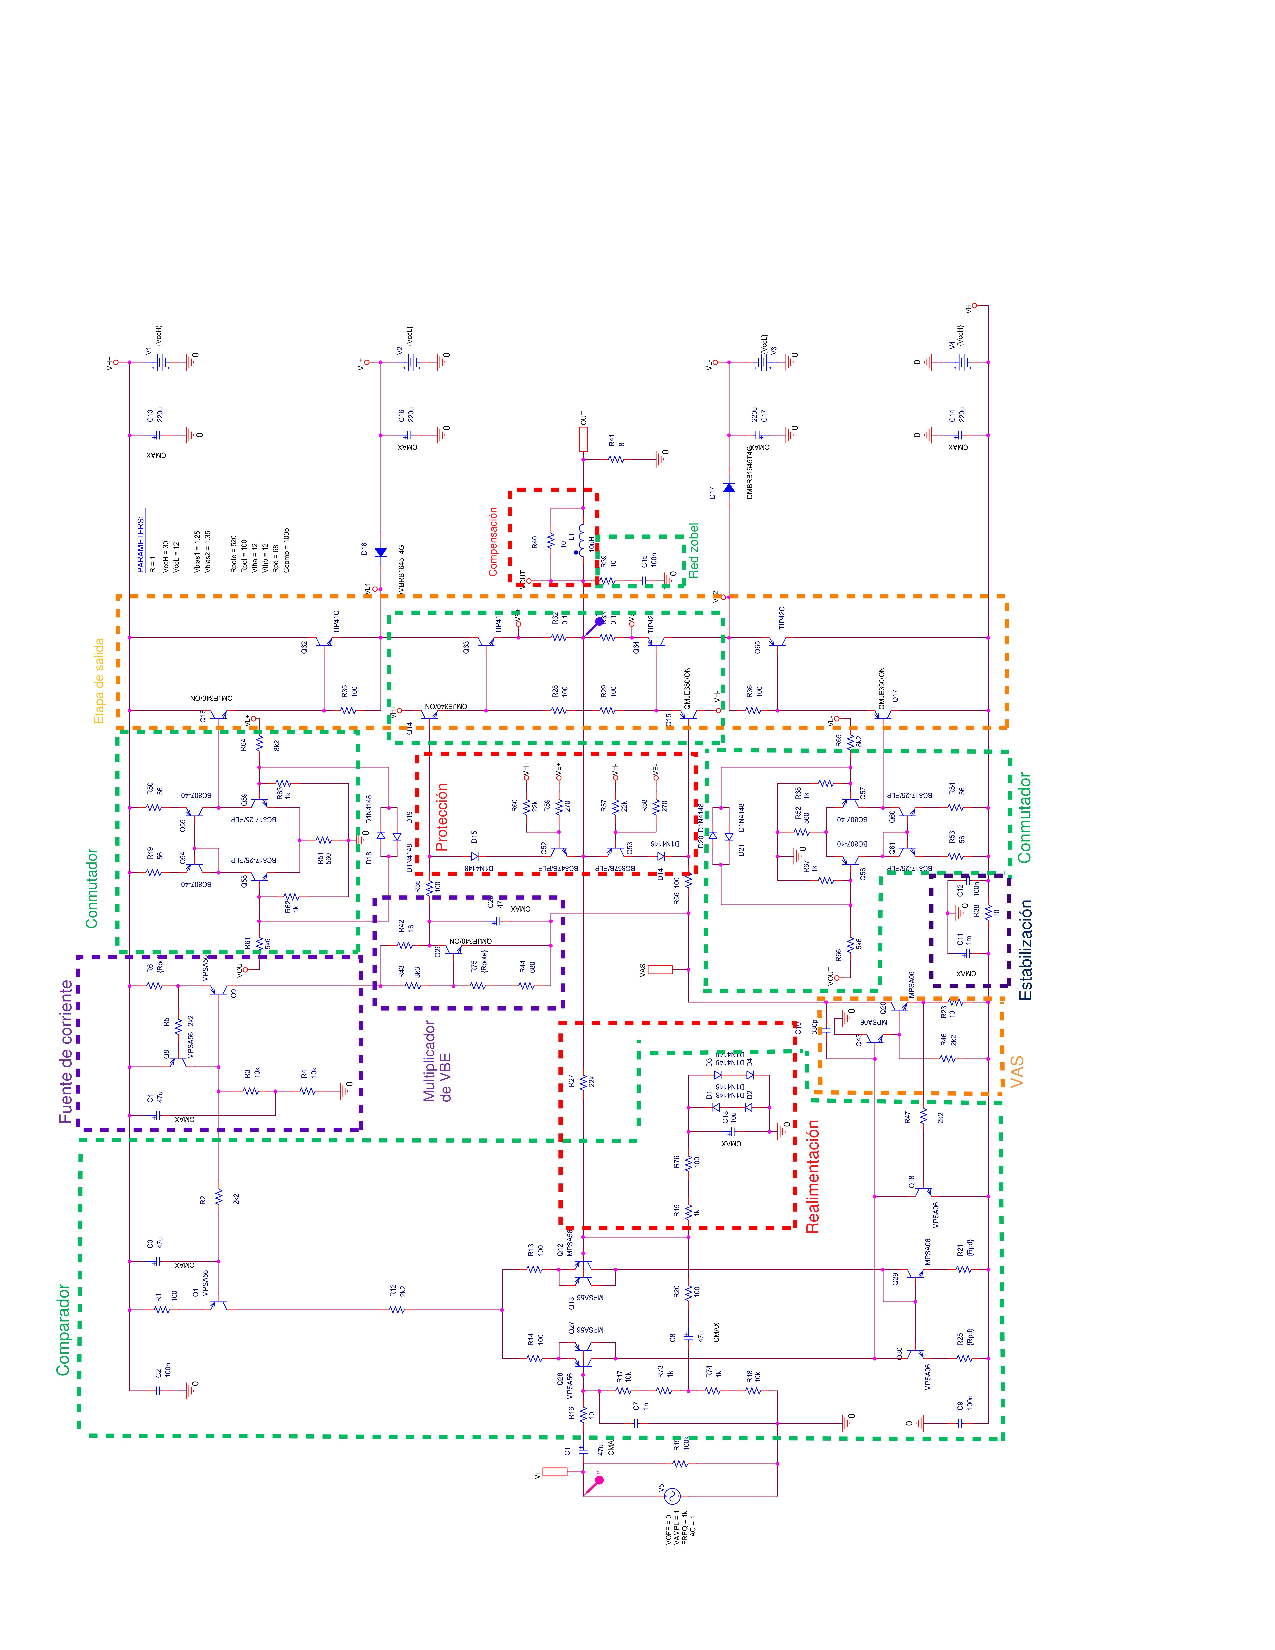
\includegraphics[angle=-90,width=1.1\textwidth, trim = 0.5cm 3.0cm 4cm 4cm]{esquema2.pdf}
	\caption{Circuito completo.}
	\label{fig.cto_completo}
\end{figure}

	% Acá se introduce al cto propuesto y después se analiza

		\section{Etapa de salida}
				La etapa de salida clase G se caracteriza principalmente por el manejo eficiente de potencia debido a que conmuta la tensión de alimentación entre dos niveles según lo requiera la señal de entrada.

	En la figura se muestra un esquema básico de la topología, denominada Clase G alternativa.  Los transistores $Q_1$ y $Q_2$ conforman la etapa interior que opera en clase B, siendo $Q3$ y $Q4$ los \textit{drivers} y $R1$ la resistencia de emisor compartida. 

	\begin{figure}[H]
		\centering
		\scalebox{0.5}{% XCircuit output "salida.tex" for LaTeX input from salida.eps
\def\putbox#1#2#3#4{\makebox[0in][l]{\makebox[#1][l]{}\raisebox{\baselineskip}[0in][0in]{\raisebox{#2}[0in][0in]{\scalebox{#3}{#4}}}}}
\def\rightbox#1{\makebox[0in][r]{#1}}
\def\centbox#1{\makebox[0in]{#1}}
\def\topbox#1{\raisebox{-0.60\baselineskip}[0in][0in]{#1}}
\def\midbox#1{\raisebox{-0.20\baselineskip}[0in][0in]{#1}}
   \scalebox{1}{
   \normalsize
   \parbox{6.61458in}{
   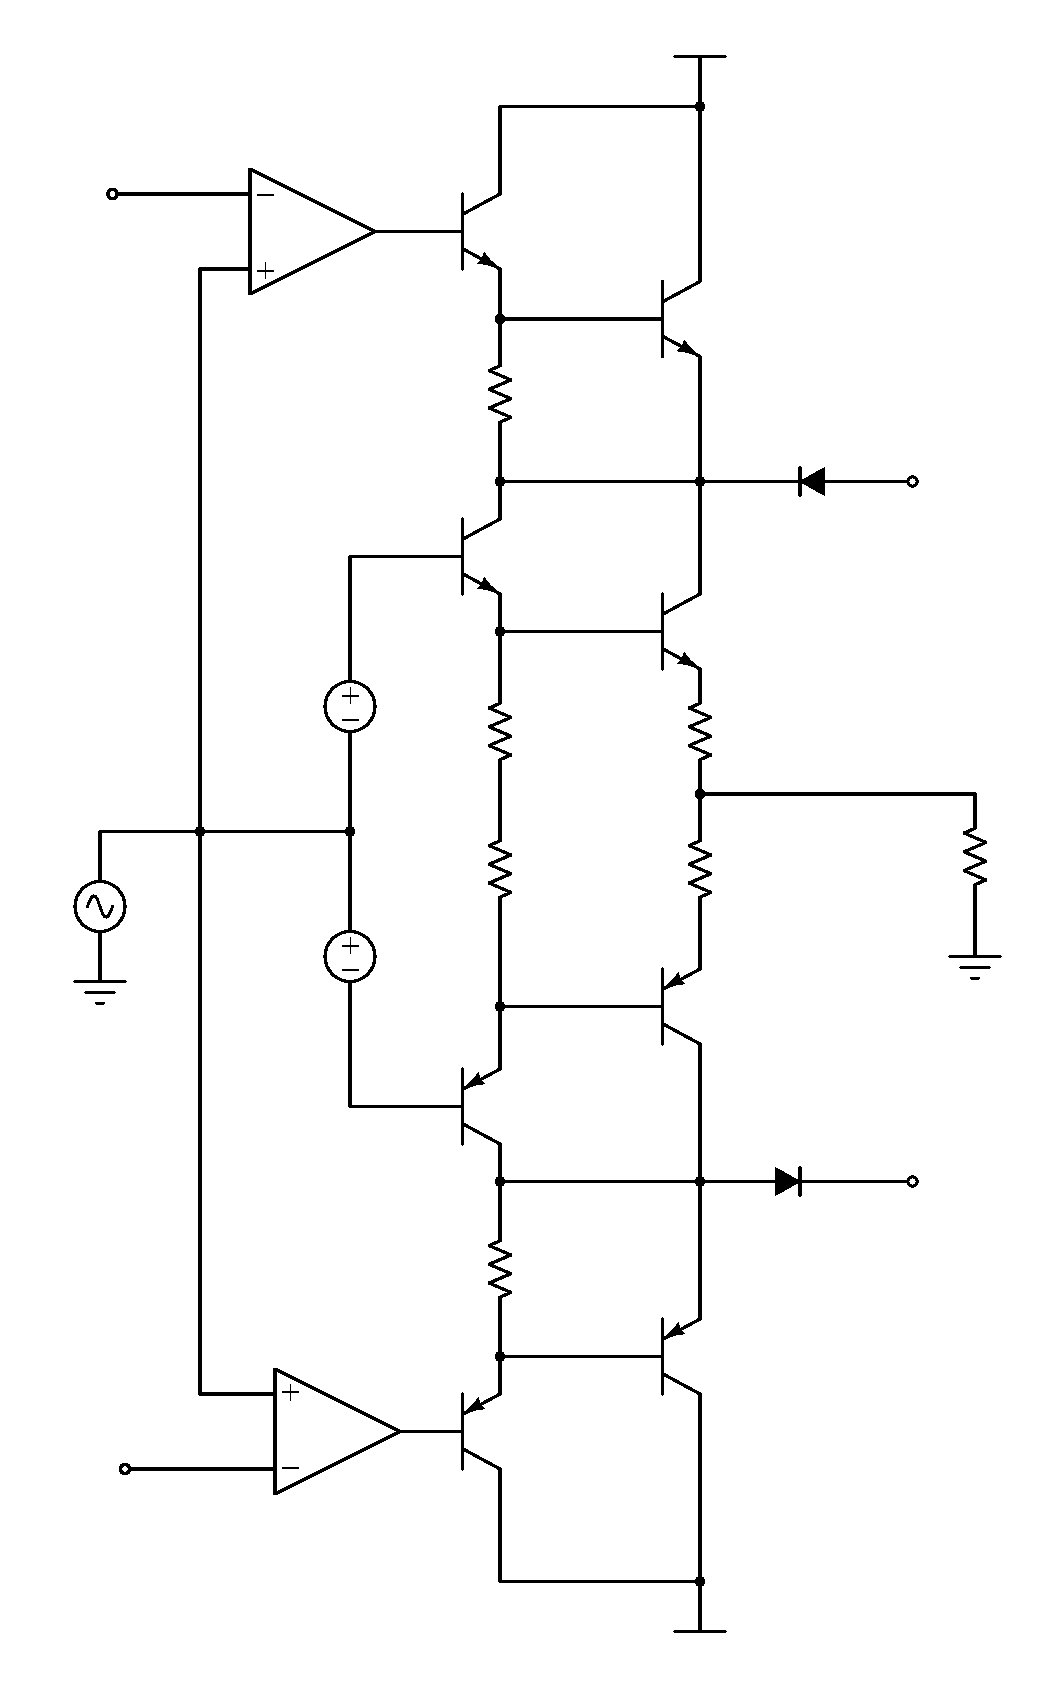
\includegraphics[scale=1]{salida}\\
   % translate x=800 y=1584 scale 0.38
   \putbox{1.39in}{6.39in}{1.20}{Vbias1}%
   \putbox{1.39in}{4.81in}{1.20}{Vbias2}%
   \putbox{5.89in}{5.39in}{1.20}{RL}%
   \putbox{4.72in}{6.22in}{1.20}{Re}%
   \putbox{4.72in}{5.31in}{1.20}{Re}%
   \putbox{4.47in}{6.89in}{1.20}{Q63}%
   \putbox{4.47in}{4.39in}{1.20}{Q64}%
   \putbox{3.14in}{7.47in}{1.20}{Q14}%
   \putbox{3.14in}{3.72in}{1.20}{Q15}%
   \putbox{3.14in}{9.56in}{1.20}{Q16}%
   \putbox{4.47in}{9.06in}{1.20}{Q62}%
   \putbox{3.14in}{1.56in}{1.20}{Q17}%
   \putbox{4.47in}{2.06in}{1.20}{Q65}%
   \putbox{0.14in}{1.31in}{1.20}{Vth-}%
   \putbox{0.06in}{9.81in}{1.20}{Vth+}%
   \putbox{4.22in}{0.06in}{1.20}{-VccH}%
   \putbox{4.22in}{10.89in}{1.20}{+VccH}%
   \putbox{6.06in}{7.89in}{1.20}{VccL+}%
   \putbox{6.06in}{3.22in}{1.20}{-VccL}%
   } % close 'parbox'
   } % close 'scalebox'
   \vspace{-\baselineskip} % this is not necessary, but looks better
}
		\caption{Etapa de salida.}
		\label{fig.salida}
	\end{figure}

	Los comparadores se encuentran conectados a la señal de entrada y a una tensión umbral Vth como referencia. Cuando la señal de entrada excede la tensión $+Vth$, el comparador (superior) hace que los transistores $Q5$ y $Q6$ se polaricen en saturación. Es decir que actúan como una llave que activa la alimentación $VccH$. A su vez el diodo $D1$ quedará polarizado en inversa ya que la tensión en el cátodo es $+VccH$, mayor que la tensión de ánodo $VccL$. Por lo tanto, el circuito queda alimentado solo mediante $+VccH$ y la potencia es manejada por dos transistores $Q6$ y $Q1$.

	De forma análoga funcionan el comparador $C2$, $Q7$, $Q8$ y $D2$ para el semicilo negativo de la señal de entrada.

	Las tensiones $Vbias1$ y $Vbias2$ permiten \textit{prepolarizar} a los transistores $Q1$ y $Q2$ con el fin de atenuar la distorsión de cruce por cero. Se deben ajustar de forma tal que la corriente de la malla de salida sea aproximadamente igual en el colector de ambos transistores ($Q1$ y $Q2$). Asimismo se debe considerar que si $ICQ$ es muy elevada se desperdicia potencia, y si es muy pequeña se obtendrá una distorsión de cruce por cero apreciable. 


\subsection{Multiplicador de $V_{BE}$}

	\begin{figure}[H]
		\centering
		\scalebox{0.5}{% XCircuit output "multiplicador.tex" for LaTeX input from multiplicador.eps
\def\putbox#1#2#3#4{\makebox[0in][l]{\makebox[#1][l]{}\raisebox{\baselineskip}[0in][0in]{\raisebox{#2}[0in][0in]{\scalebox{#3}{#4}}}}}
\def\rightbox#1{\makebox[0in][r]{#1}}
\def\centbox#1{\makebox[0in]{#1}}
\def\topbox#1{\raisebox{-0.60\baselineskip}[0in][0in]{#1}}
\def\midbox#1{\raisebox{-0.20\baselineskip}[0in][0in]{#1}}
   \scalebox{1}{
   \normalsize
   \parbox{4.18229in}{
   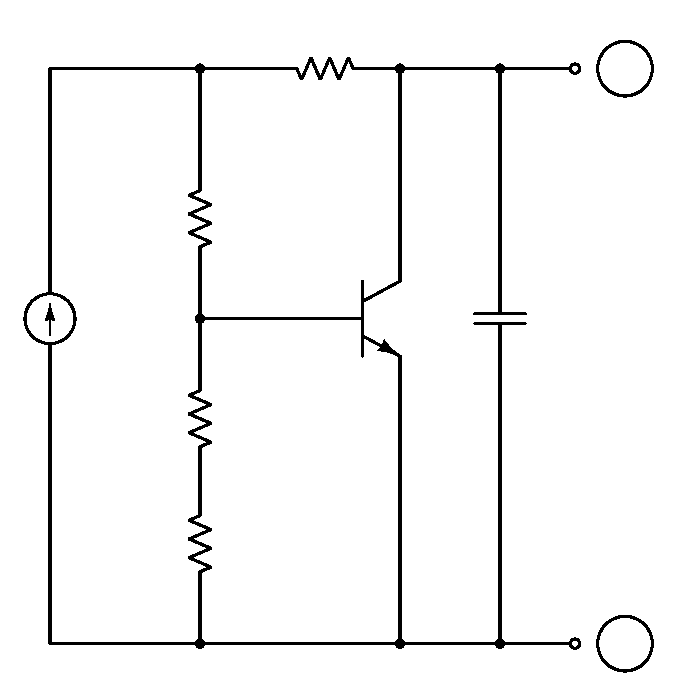
\includegraphics[scale=1]{multiplicador}\\
   % translate x=672 y=611 scale 0.38
   \putbox{3.56in}{2.32in}{1.20}{C20}%
   \putbox{2.47in}{2.32in}{1.20}{Q26}%
   \putbox{0.56in}{3.07in}{1.20}{R43}%
   \putbox{0.72in}{1.74in}{1.20}{Rp}%
   \putbox{0.64in}{0.82in}{1.20}{R44}%
   \putbox{1.89in}{4.24in}{1.20}{R42}%
   \putbox{4.06in}{4.07in}{1.20}{\centbox{\midbox{1,1}}}%
   \putbox{4.06in}{0.24in}{1.20}{\centbox{\midbox{-1,1}}}%
   \putbox{0.47in}{2.32in}{1.20}{Ipol}%
   \putbox{1.97in}{3.74in}{1.20}{$10 \Omega$}%
   \putbox{1.47in}{3.07in}{1.20}{$3,3 k\Omega$}%
   \putbox{1.39in}{0.82in}{1.20}{$680 \Omega$}%
   \putbox{1.39in}{1.65in}{1.20}{$1 k\Omega$}%
   } % close 'parbox'
   } % close 'scalebox'
   \vspace{-\baselineskip} % this is not necessary, but looks better
}
		\caption{Multiplicador de $V_{BE}$.}
		\label{fig.multiplicador}
	\end{figure}

	La resistencia $R_{3M}$ se anexa para mejorar la independencia de la tensión $V_{BE}$ con la corriente de polarización.

	\begin{equation}
		\centering
		V_M = \left( \frac{R_{1M}}{R_{1M} + R_{2M}} +1 \right) \cdot V_{BE} - I_C \cdot R_{3M} \approx  \left( \frac{R_{1M}}{R_{1M} + R_{2M}} +1 \right) \cdot V_{BE}
	\end{equation}

	 Considerando un valor de $V_{BE} \approx \SI{0.5}{\volt}$

	 \begin{equation}
	 	\centering
		\frac{\SI{2.2}{\volt}}{\SI{0.5}{\volt}} -1 = \frac{R_{1M}}{R_{2M}} \implies \boxed{R_{1M} = \num{3,4} \cdot R_{2M}}
	\end{equation}
	Se eligen los resistores comerciales $R_{1M} = \SI{3.3}{\kilo\ohm}$, $R_{2M} = \SI{680}{\ohm}$ y un potenciómetro de $\SI{1}{\kilo\ohm}$. 


\subsection{Comparadores}

	\begin{figure}[H]
		\centering
		\scalebox{0.5}{% XCircuit output "comparador.tex" for LaTeX input from comparador.eps
\def\putbox#1#2#3#4{\makebox[0in][l]{\makebox[#1][l]{}\raisebox{\baselineskip}[0in][0in]{\raisebox{#2}[0in][0in]{\scalebox{#3}{#4}}}}}
\def\rightbox#1{\makebox[0in][r]{#1}}
\def\centbox#1{\makebox[0in]{#1}}
\def\topbox#1{\raisebox{-0.60\baselineskip}[0in][0in]{#1}}
\def\midbox#1{\raisebox{-0.20\baselineskip}[0in][0in]{#1}}
   \scalebox{1}{
   \normalsize
   \parbox{7.08333in}{
   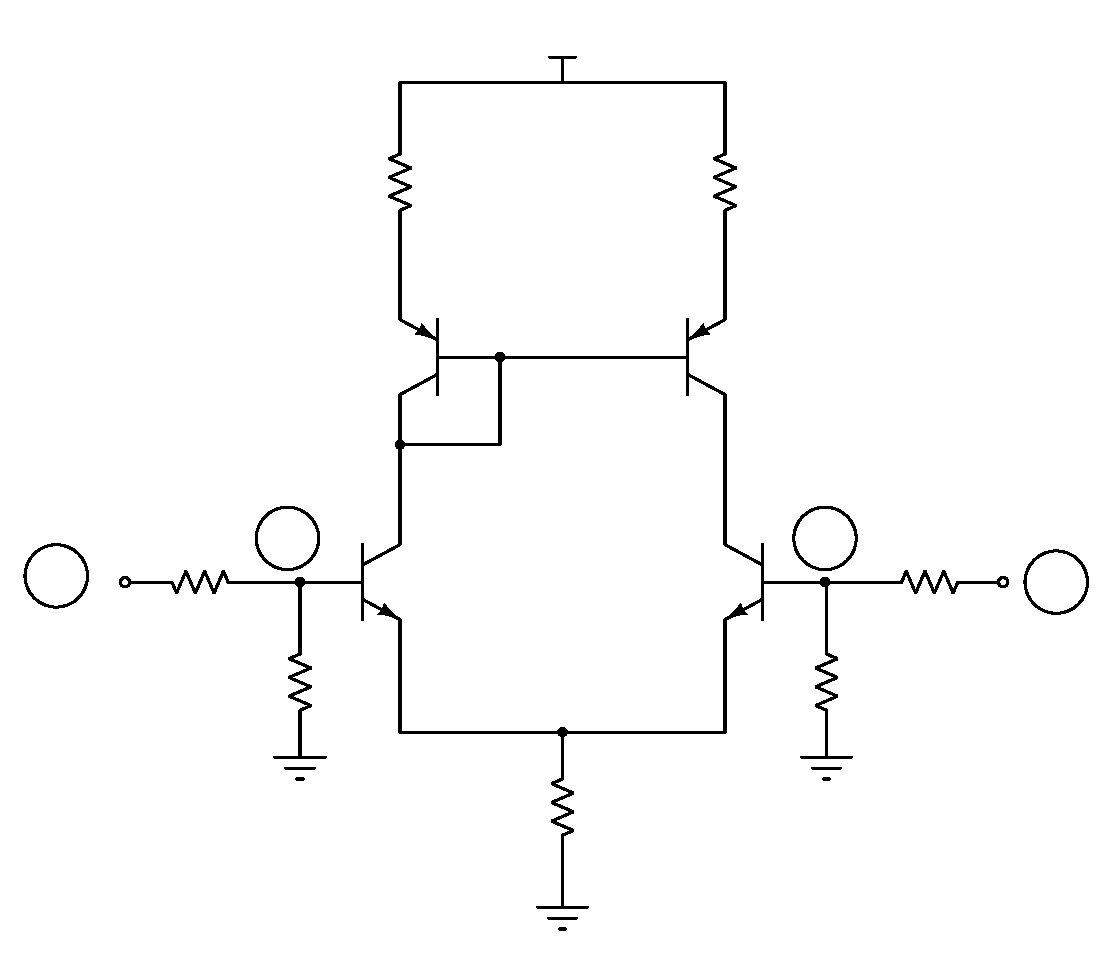
\includegraphics[scale=1]{comparador}\\
   % translate x=928 y=636 scale 0.38
   \putbox{2.58in}{2.33in}{1.20}{Q9}%
   \putbox{4.45in}{2.29in}{1.20}{Q10}%
   \putbox{2.37in}{3.81in}{1.20}{Q11}%
   \putbox{4.66in}{3.81in}{1.20}{Q12}%
   \putbox{3.35in}{5.95in}{1.20}{+VccH}%
   \putbox{0.14in}{2.33in}{1.20}{Vo}%
   \putbox{3.18in}{0.83in}{1.20}{Rec}%
   \putbox{1.10in}{2.54in}{1.20}{R1}%
   \putbox{1.47in}{1.70in}{1.20}{R2}%
   \putbox{5.97in}{2.49in}{1.20}{R3}%
   \putbox{5.01in}{1.66in}{1.20}{R4}%
   \putbox{2.18in}{5.04in}{1.20}{R5}%
   \putbox{4.35in}{4.99in}{1.20}{R6}%
   \putbox{1.64in}{2.58in}{1.20}{Vo'}%
   \putbox{5.18in}{2.58in}{1.20}{Vth'}%
   \putbox{6.76in}{2.33in}{1.20}{Vth}%
   \putbox{2.76in}{5.04in}{1.20}{56}%
   \putbox{4.93in}{5.04in}{1.20}{56}%
   \putbox{1.10in}{2.08in}{1.20}{5,6k}%
   \putbox{2.06in}{1.70in}{1.20}{1k}%
   \putbox{5.51in}{1.70in}{1.20}{1k}%
   \putbox{5.89in}{2.08in}{1.20}{8,2k}%
   \putbox{3.81in}{0.83in}{1.20}{560}%
   } % close 'parbox'
   } % close 'scalebox'
   \vspace{-\baselineskip} % this is not necessary, but looks better
}
		\caption{Comparador.}
		\label{fig.comparador}
	\end{figure}

	Se propone la configuración de par diferencial de la figura para implementar los comparadores. Se utiliza una fuente de corriente espejo para lograr mayor estabilidad. En vez de comparar con la señal proveniente de la etapa VAS, se compara con la señal de salida $V_{o}$ para evitar cargar la VAS con la resistencia de entrada que presenta el par diferencial ($2\cdot r_\pi$). La señal de salida no resulta alterada por tratarse de un colector común que es separador de impedancias.
	Por otra parte, es difícil lograr en la práctica que los transistores que conforman el par diferencial manejen una excursión de tensión de hasta \SI{30}{\volt}, por lo que se utiliza un divisor resistivo en ambas bases de los transistores para atenuar la amplitud de tensión. Es conveniente que la tensión de referencia $Vth'$ sea levemente menor que la prevista con el fin de contrarrestar el retardo de tiempo del comparador.

\begin{equation}
	\centering
	V_{th}' = V_{th} \cdot \frac{R_4}{R_4 + R_3} \implies \SI{1.5}{\volt} = \SI{12}{\volt} \cdot \frac{R_4}{R_4 + R_3} \implies \boxed{R_3 = 7 \cdot R_4}
\end{equation}

\begin{equation}
	\centering
	V_o' = V_o \cdot \frac{R_2}{R_2 + R_1} \implies \SI{2}{\volt} = \SI{12}{\volt} \cdot \frac{R_2}{R_2 + R_1} \implies \boxed{R_1 = 5 \cdot R_2}
	\end{equation}

	El valor de la resistencia de emisor $R_{ec}$ se elige en función de la máxima tensión posible en $V_o$ y la corriente que circularía en reposo. Con $R_ec = \SI{500}{\ohm}$ se obtiene:

	\begin{equation}
		\centering
		I_{e,max} = \frac{ \SI{1.3}{\volt} }{ \SI{500}{\ohm} } = \SI{2.6}{\milli\ampere}
	\end{equation}

	\begin{equation}
		I_{e,pol} = \frac{ \SI{0.8}{\volt} }{ \SI{500}{\ohm} } = \SI{1.6}{\milli\ampere} \implies \SI{1.28}{\milli\watt}
	\end{equation}



%		\section{Polarización}\label{sec:pol}
%			\input{III1_polarizacion.tex}
%		
%		\section{Ganancia de lazo}\label{sec:gan_lazo}
%			\input{III2_gan_lazo.tex}
%		
%		\section{Ganancia global}\label{sec:gan_global}
%			\input{I3_gan_global.tex}
%	
%		\section{Máxima potencia sobre la carga}\label{sec:pot_carga}
%			\input{I4_pot_carga.tex}
%	
%		\section{Impedancia de entrada}\label{sec:zi}
%			\input{I5_zi.tex}
%	
%		\section{Impedancia de salida}\label{sec:zo}
%			\input{I6_zo.tex}
%		
%		\section{Factor de amortiguamiento}\label{sec:amort}
%			\input{I7_amortiguamiento.tex}
%	
%		\section{Máxima tensión pico sobre la carga}\label{sec:pico_carga}
%			\input{I8_pico_carga.tex}
%		\pagebreak	
%		\section{Máxima eficiencia del amplificador}\label{sec:eficiencia}
%			\input{I9_eficiencia.tex}
%		\pagebreak	
%		\section{Disipadores}\label{sec:disipadores}
%			\input{I10_disipadores.tex}

	\part{Diseño del circuito impreso - \emph{PCB}}\label{part:pcb}

		\section{Elección de componentes}\label{sec:componentes}
			En las Tablas \ref{tab:lst_tr}, \ref{tab:lst_cap} y \ref{tab:lst_resist} se detallan todos los componentes necesarios para la implementación del circuito, teniendo en cuenta los valores comerciales disponibles.

\begin{table}[h!]
	\centering
	\begin{tabular}{cccc}
		\toprule
		Código & Nombre & Características & Cantidad \\
		\midrule
		\texttt{2SC5198} & Q62, Q63 & NPN & 2 \\
		\texttt{2SA194} & Q64, Q65 & PNP & 2 \\ 
		\texttt{MJE340} & Q14, Q16, Q26 & NPN & 3 \\
		\texttt{MJE350} & Q15, Q17 & PNP & 2 \\
		\texttt{MPSA56} & Q1, Q8, Q9, Q12, Q13, Q27, Q28& PNP   & 7 \\ 
		\texttt{MPSA06} & Q30, Q29, Q43, Q20 & NPN  & 4 \\
		\texttt{BC817}  & Q56, Q59, Q61, Q60 & NPN SMD & 4 \\
		\texttt{BC807}  & Q54, Q55, Q56, Q57 & PNP SMD & 4 \\
		\texttt{BC847}  & Q52 & NPN SMD & 1  \\
		\texttt{BC857}  & Q53 & PNP SMD & 1 \\
		\midrule
		\texttt{1N4148} & D1,2,3,4,14,15,18,19,20,21  & Diodo de alta conmutación & 10 \\
		\texttt{MBRB1645T4G} & D16, D17 & Diodo Schottky & 2 \\
		\bottomrule
	\end{tabular}
	\caption{Transistores y diodos utilizados en el circuito.}
	\label{tab:lst_tr}
\end{table}

\begin{table}[h!]
	\centering
	\begin{tabular}{cccc}
		\toprule
		Valor & Nombre & Tecnología & Cantidad \\
		\midrule
		\SI{10}{\micro\farad} & C18 & Electrolítico & 1 \\	 
		\SI{47}{\micro\farad} & C1, C4, C20, & Electrolítico & 3 \\
		\SI{1}{\milli\farad} & C11 & Electrolítico & 1 \\
		\SI{100}{\nano\farad} & C2, C9, C12, C15 & Poliéster & 3 \\
		\SI{1}{\nano\farad} & C7 & Poliéster & 1 \\
		\SI{330}{\pico\farad} & C10 & Cerámico & 1 \\
		\bottomrule
	\end{tabular}
	\caption{Capacitores y tecnología de los mismos para la implementación del circuito.}
	\label{tab:lst_cap}
\end{table}

\begin{table}[h!]
	\centering
	\begin{tabular}{cccc}
		\toprule
		Valor & Nombre & Tecnología & Cantidad \\
		\midrule
		\SI{0.1}{\ohm} & R32, R33 & Alambre, 5W & 2 \\
		\SI{10}{\ohm} & R39 & Alambre, 5W & 1 \\		
		\SI{10}{\ohm} & R38 & Metalfilm 1W & 1 \\
		\SI{100}{\ohm} & R28, R29, R35, R36 & Metalfilm 1W & 4 \\
		\SI{22}{\kilo\ohm} & R27 & Metalfilm, 1W & 1 \\
		\SI{10}{\ohm} & R16, R23 & SMD 0805 & 2 \\
		\SI{15}{\ohm} & R42 & SMD 0805 & 1 \\
		\SI{56}{\ohm} & R49, R50, R53, R54 & SMD 0805 & 4 \\
		\SI{68}{\ohm} & R21, R25 & SMD 0805 & 2 \\
		\SI{100}{\ohm} & R1,13,14,20,76 & SMD 0805 & 5 \\
		\SI{270}{\ohm} & R59, R60 & SMD 0805 & 2 \\ 
		\SI{560}{\ohm} & R51, R62 & SMD 0805 & 2 \\
		\SI{680}{\ohm} & R44 & SMD 0805 & 1\\
		\SI{1}{\kilo\ohm} & R73, R74, R15, R62, R63, R67, R68  & SMD 0805 & 7 \\
		\SI{2.2}{\kilo\ohm} & R5, R47 & SMD 0805 & 2 \\ 
		\SI{3.3}{\kilo\ohm} & R43 & SMD 0805 & 1 \\
		\SI{5.6}{\kilo\ohm} & R61, R66 & SMD 0805 & 2 \\
		\SI{8.2}{\kilo\ohm} & R64, R65 & SMD 0805 & 2 \\
		\SI{10}{\kilo\ohm} & R17, R18 & SMD 0805 & 2 \\
		\SI{100}{\kilo\ohm} & R19 & SMD 0805 & 2 \\
		\bottomrule
	\end{tabular}
	\caption{Lista de resistencias requeridas para el circuito.}
	\label{tab:lst_resist}
\end{table}


		\section{Criterios de Ruteo}\label{sec:ruteo}
			\begin{itemize}
	\item Las fuentes de alimentación se se colocaron lo más cerca posible de la etapa de salida, ya ésta es la que maś corriente consume.
	\item Sabiendo que la corriente máxima que puede circular por la salida es de \SI{3.5}{\ampere}, una pista de 75 mills resulta sufifiente para las pistas de potencia.
	\Flor{Completar}
	\item Pistas de baja potencia de mills.
	\item El camino entre la salida y realimentación se colocó lo más cerca posible, lo mismo entre el el comparador y la salida, debido a que se reuiere velocidad. 
	\item No se dejaron espacios vacíos, sino que se dejaron con cobre y conectados a tierra para así obtener islas de masa.
	\item Los transistores de entrada se colocaron lo más cercanos posible para obtener un buen acoplamiento térmico.
	\item Se verificó que no se formen espiras, ya que se comportarían como inductancias.
	\item Se procuró que las pistas no posean esquinas con puntas ó ángulos agudos para evitar interferencias y facilitar la fabricación.

\end{itemize}


	\part{Análisis por simulación}\label{part:sim}
		
		\section{Etapa de salida}\label{sec:sim_salida}
			\begin{figure}[H]
	\centering
	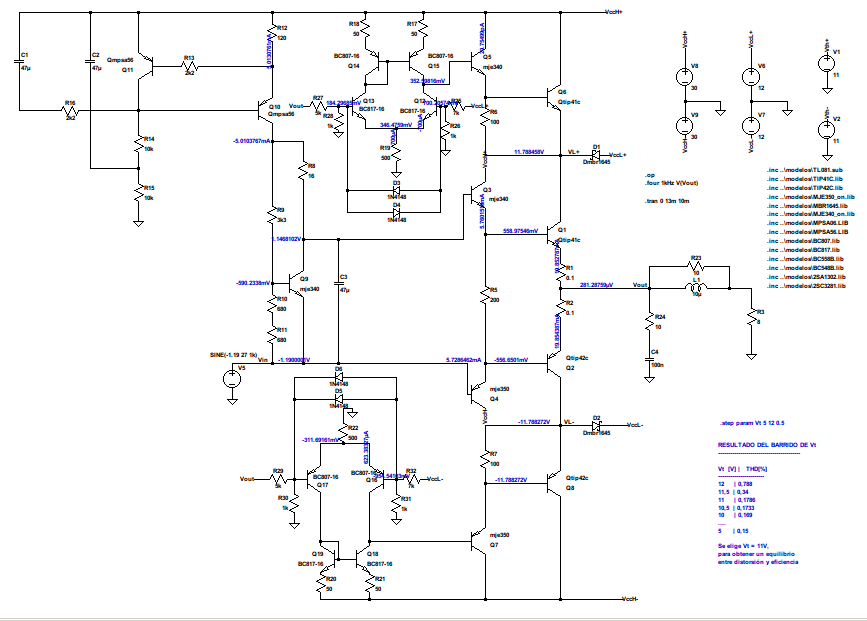
\includegraphics[scale=0.5]{sim_esq_salida.png}
	\caption{Etapa de salida.}
	\label{fig.sim_esq_salida}
\end{figure}


\begin{figure}[H]
	\centering
	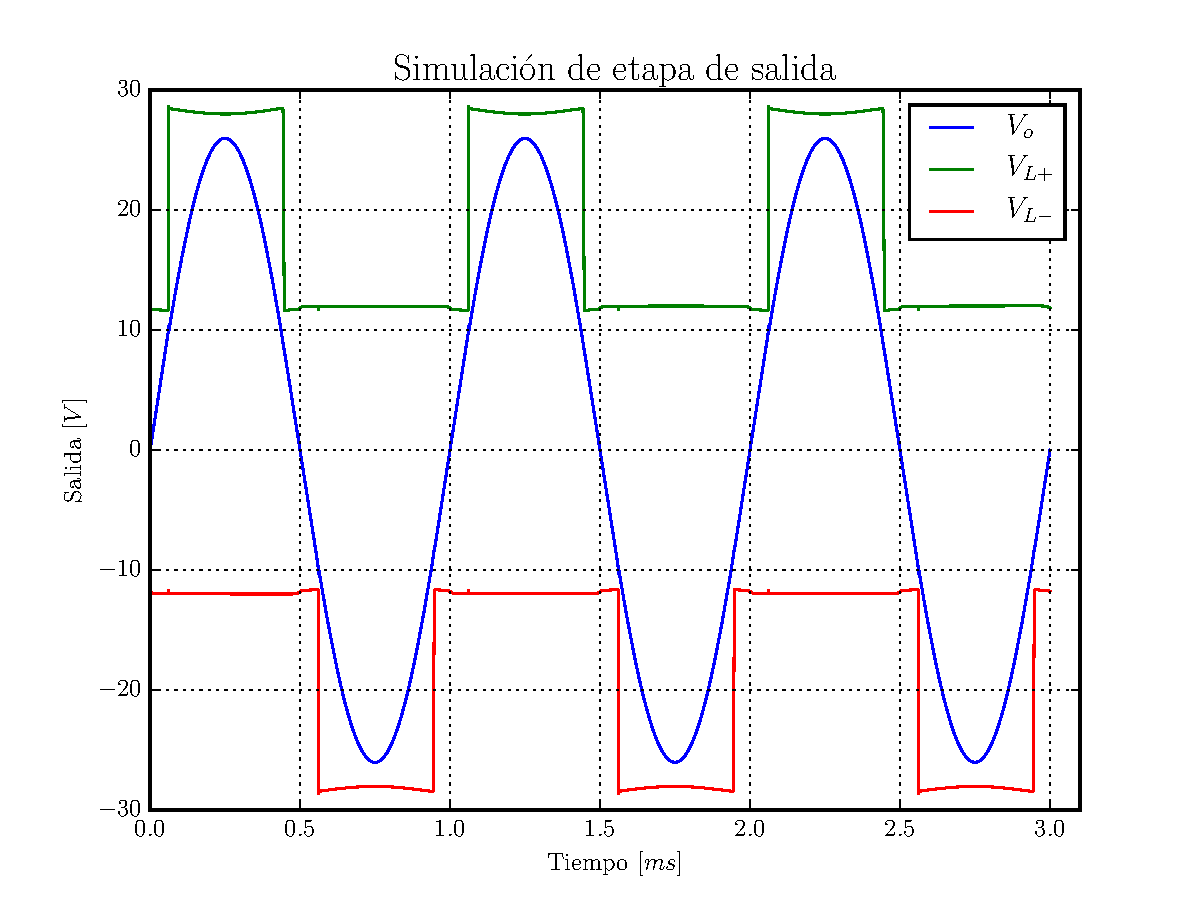
\includegraphics[scale=0.5]{sim_etapa_salida.pdf}
	\caption{Simulación de la etapa de salida $\mathrm{THD} =0.154021\%$ .}
	\label{fig.salida}
\end{figure}


		\section{Etapa de amplificación de tensión}{\label{sec:sim_vas_pd}
			
\begin{figure}[H]
	\centering
	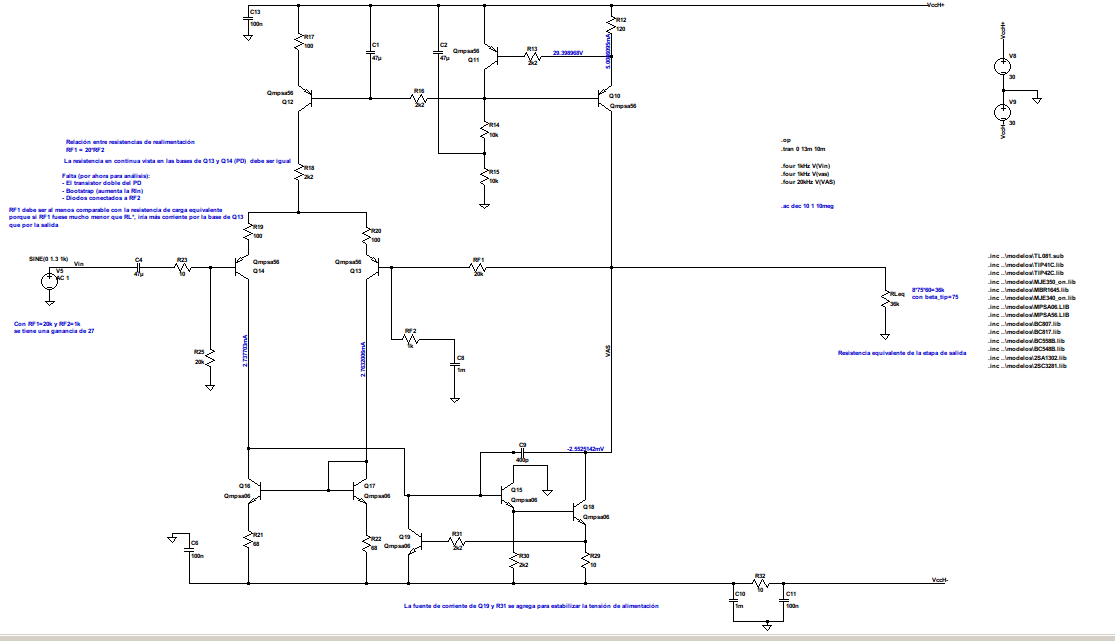
\includegraphics[scale=0.5]{sim_esq_vas.png}
	\caption{Primeras dos etapas.}
	\label{fig:sim_salida}
\end{figure}

\begin{figure}[H]
	\centering
	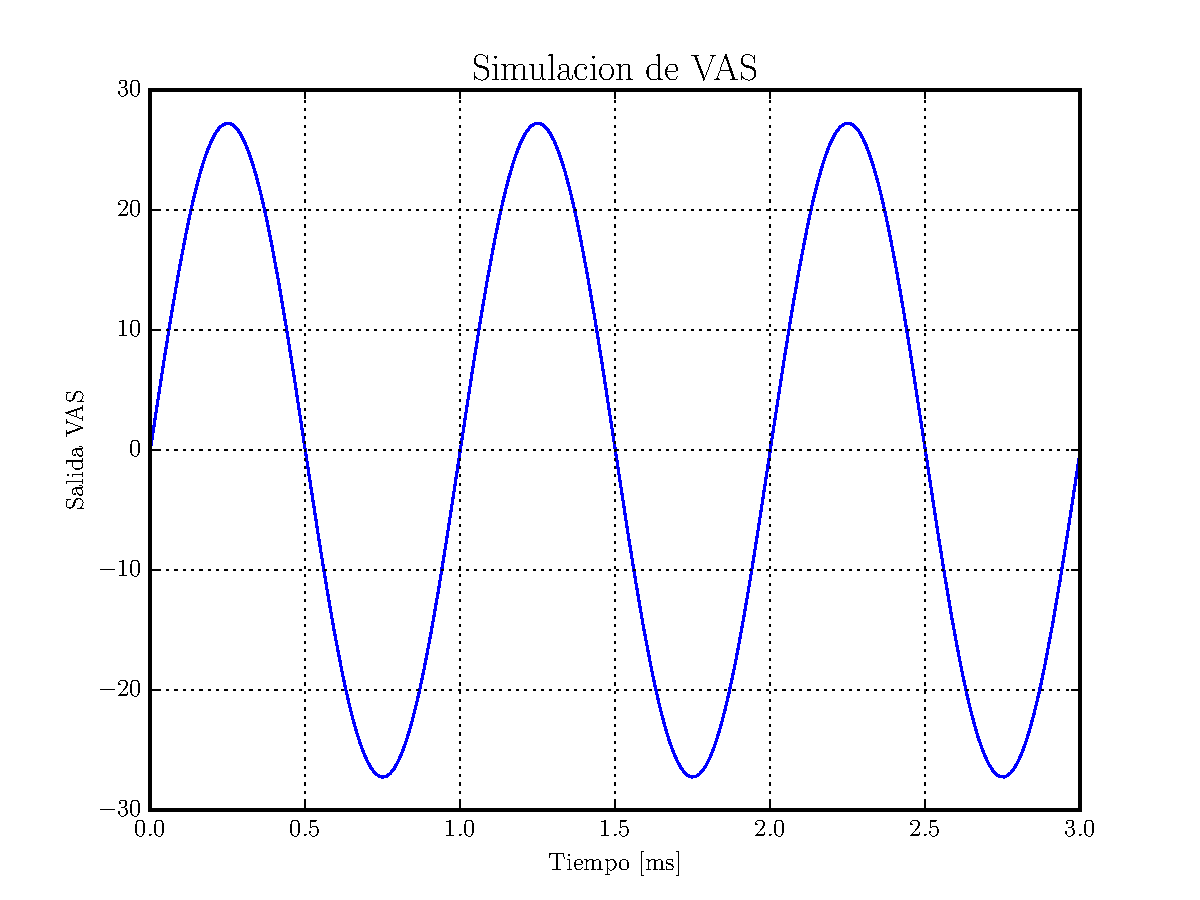
\includegraphics[scale=0.5]{sim_vas.pdf}
	\caption{Salida de la etapa VAS $\mathrm{THD}=0,000205\%$.}
	\label{fig:sim_vas}
\end{figure}

\begin{figure}[H]
	\centering
	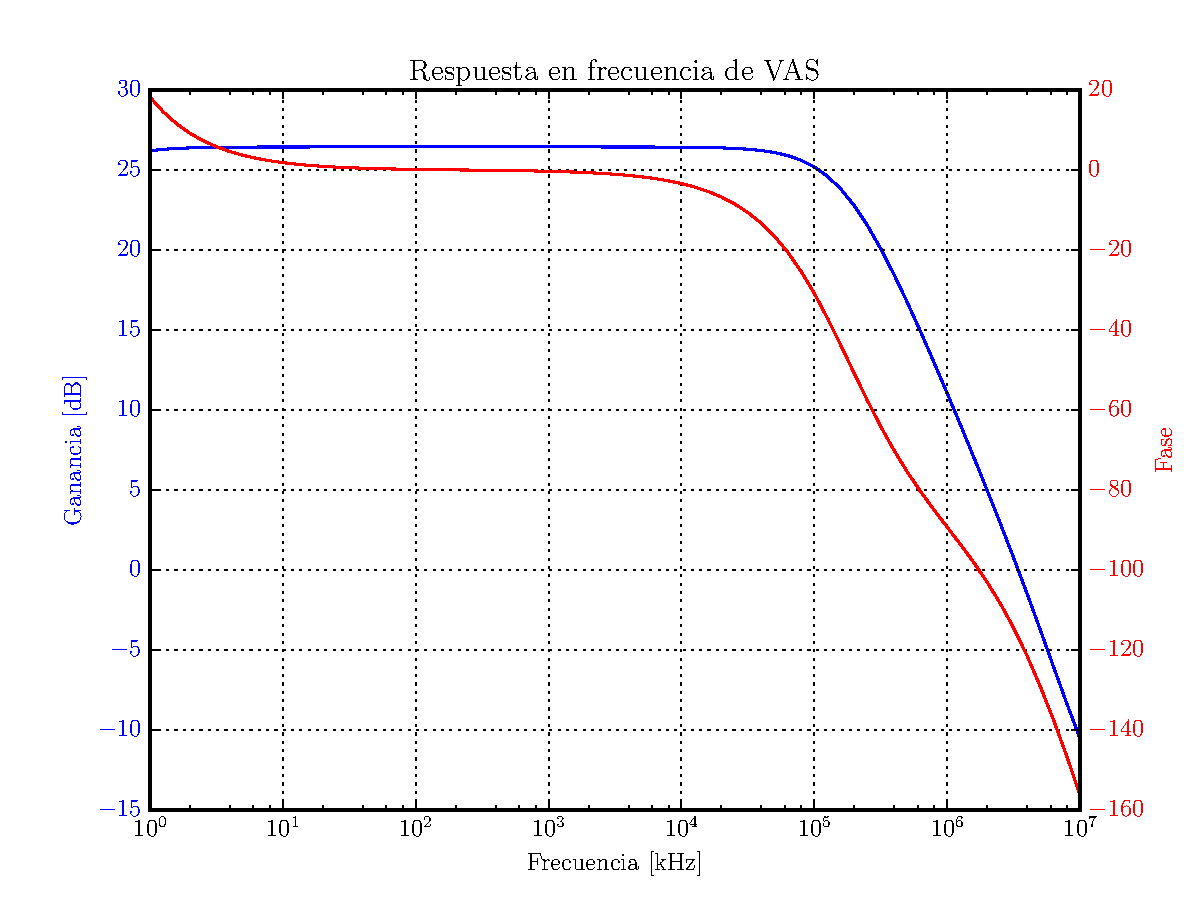
\includegraphics[scale=0.5]{sim_vas_bode.pdf}
	\caption{Respuesta en frecuencia de la etapa VAS.}
	\label{fig:sim_bode_vas}
\end{figure}

A partir de la figura \ref{fig:sim_bode_vas} se observa que el margen de fase resulta ser de $\SI{60}{\degree}$, se obtuvo ajustando el valor del capacitor de compensación $C2$ en $\SI{400}{\pico\farad}$.


%		\section{Polarización}\label{sec:sim_pol}
%			\input{V_polarizacion.tex}
%
%		\section{Impedancia de entrada}\label{sec:sim_zi}
%			\input{II2_zi.tex}
%
%		\section{Impedancia de salida}\label{sec:sim_zo}
%			\input{II3_zo.tex}
%
%		\section{Respuesta en frecuencia}\label{sec:sim_rta_frec}
%			\input{II4_rta_frec.tex}
%
%		\section{Ancho de banda de potencia}\label{sec:sim_bw}
%			\input{II5_bw.tex}
%
%		\section{Respuesta al escalón}\label{sec:sim_escalon}
%			\input{II6_escalon.tex}
%	
%		\section{Margen de fase}\label{sec:sim_fase}
%			\input{II7_fase.tex}
%		\pagebreak
%		\section{Distorsión armónica}\label{sec:sim_thd}
%			\input{II8_thd.tex}
%		
%		\section{Distorsión por intermodulación}\label{sec:sim_intermod}
%			\input{II9_intermod.tex}
%		\pagebreak
%		\section{Rechazo de Ruido de la Fuente de Alimentación}\label{sec:sim_psnr}
%			\input{II10_psrr.tex}
%	\pagebreak

	\part{Construcción del prototipo}\label{part:construccion}
		\Juan{Ver pdf ''Grupo01\_informe\_final`` como referencia}
%		\input{VI}

	\part{Medición del prototipo}\label{part:mediciones}
%		\input{VII}

	\part{Conclusiones}\label{part:conclusiones}
		%En el presente informe se logró analizar el circuito \textit{Turner 730}, obteniéndose resultados semejantes por inspección y simulación.

%La respuesta en frecuencia obtenida resultó ser plana dentro del rango de frecuencias audibles e invariante a la potencia disipada. 

%La eficiencia máxima del circuito (71,2\%) resultó cercana a la ideal (78,5\%), aunque nunca llegará a dicho valor ya que el nodo de salida no puede alcanzar los \SI{30}{\V} (por las caídas de tensión de control de los transistores equivalentes).

%La utilización de un par complementario (\textit{Sziklai}) en vez de un \textit{Darlington} reduce notablemente la distorsión armónica. Pero en el cirucito \textit{Turner 730}, uno de los transistores de etapa de salida es \textit{Darlington}. Esta elección de diseño puede deberse a que en los años 70 los transistores \textit{NPN} y \textit{PNP} no presentaban tanta simetría como hoy en día.


	En el presente informe se logró diseñar un amplificador de audio clase G alternativa, obteniéndose resultados por simulación similares a las especificaciones definidas. La comparación se resume en la Tabla \ref{tab.resultados}. La tensión máxima posible sin distorsión logró llegar a \SI{26.1}{\volt} por simulación, esto produce una potencia sobre la carga de \SI{42.25}{\watt}, por lo que se tiene cierta tolerancia con respecto a la potencia nominal especificada.\\
	\indent A su vez las mediciones realizadas los días \texttt{4/12/18} y \texttt{5/12/18} de las primeras 2 etapas coinciden con los valores obtenidos en el análisis preliminar.





	\part{Bibliografía}\label{part:bibliografia}
		\input{IX_bibliografia.tex}

	\appendix
	\section{Listado de componentes}
		\input{A_listado_comp.tex}
\end{document}
